\subsection{Chroma SCPI Commands Example Programs}
The following programming is a raw program that we can do through NI drivers. 

\paragraph{Example 1:} The following commands in example 1 simulate a BMS containing 16 independent batteries with sampling 10ms and current range to 5A. The initial voltage of the 16 batteries is 3.8V/2A and remains 0.5 second after output. When the voltage changes to 4.2V/3A and remains for
0.5 second, it reports the first 100 records of battery 1 and 2, and then turn off the output'\cite{Chroma_UserManual}.
\\\\
\noindent $*IDN?$ \\
$SYSTem:FRAME:STATe?$ 0\\
$SYST:FRAME?$ 0\\
$SYST:FRAME:CHAN:STAT?$ 0\\
$SYST:FRAME:CHAN:NUMB?$ 0 \\
$SYST:ERR?$\\
$SYSTem:ERRor?$\\ 
$SYST:FRAME:PROT:CLE$\\
$SIM:CONF:BMS:NUMB$ 1\\ 
$SIM:CONF:BMS:NUMB?$ \\
$SIM:CONF:SAMP:TIME$ 10\\ 
$SIM:CONF:SAMP:TIME?$\\ 
$SIM:CONF:CELL:NUMB$ 1,16\\
$SIM:CONF:CELL:NUMB?$ 1\\
$SIM:CONF:CELL:PARA$ 1,1,16,1,2\\
$SYSTem:ERRor?$\\ 
$SIM:PROG:CELL$ 1,1,1,16,3.8,2\\
$SIM:OUTP ON$\\
$SYSTem:ERRor?$ \\
$SIM:OUTP?$\\
$*D$ 500\\
$SIM:PROG:CELL$ 1,1,1,16,4.2,3\\
$SYSTem:ERRor?$\\ 
$SIM:OUTP:IMM$\\
$SYSTem:ERRor?$\\
$*D$ 500\\
$SIM:REP:CELL:REC:DATA?$ 1,1,1,100\\
$SIM:REP:CELL:REC:DATA?$ 1,2,1,100\\
$SIM:OUTP OFF$\\
$SYSTem:ERRor? SIM:OUTP?$\\


\paragraph{Example 2:} The following commands in example 2 simulate a BMS containing 16 independent batteries that are paralleled into 8 separate batteries with sampling 10ms and a current range of 5A. The voltage of the 8 batteries is 4.2 V/2A, and it performs measurement 1 second after output. It returns the instant voltage, current and protection status of BMS 1 8 batteries, and turns off the output after 10 seconds.
\\\\
$*IDN?$ \\
$SYSTem:FRAME:STATe?$ 0\\
$SYST:FRAME?$ 0\\
$SYST:FRAME:CHAN:STAT?$ 0\\
$SYST:FRAME:CHAN:NUMB?$ 0 \\
$SYST:ERR?$\\
$SYSTem:ERRor?$\\ 
$SYST:FRAME:PROT:CLE$\\
$SIM:CONF:BMS:NUMB$ 1\\ 
$SIM:CONF:BMS:NUMB?$ \\
$SIM:CONF:SAMP:TIME$ 10\\ 
$SIM:CONF:SAMP:TIME?$\\ 
$SIM:CONF:CELL:NUMB$ 1,16\\
$SIM:CONF:CELL:NUMB?$ 1\\
$SIM:CONF:CELL:PARA$ 1,1,8,2,2\\
$SIM:OUTP ON$\\
$SYSTem:ERRor?$ \\
$SIM:OUTP?$\\
$*D $1000\\
$SIM:MEAS:BMS:VOLT?$ 1\\
$SIM:MEAS:BMS:CURR?$ 1\\
$SIM:MEAS:BMS:PROT?$ 1\\
$*D $10000\\
$SIM:OUTP OFF$\\
$SYSTem:ERRor?$\\
$SIM:OUTP?$\\


\begin{figure}[h]
	\centering
	\subfigure[4 Channel keysight N6705 Power Supply]{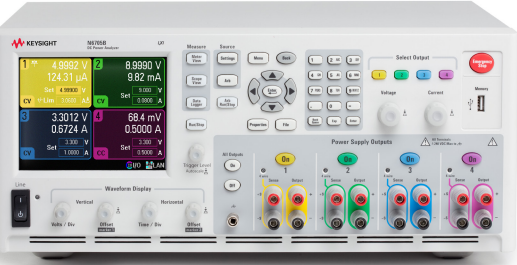
\includegraphics[width=0.3\textwidth]{Chap06/Figures/keysight_n6705.PNG}}
    \qquad
	\subfigure[Chroma Output Wiring to the BMS]{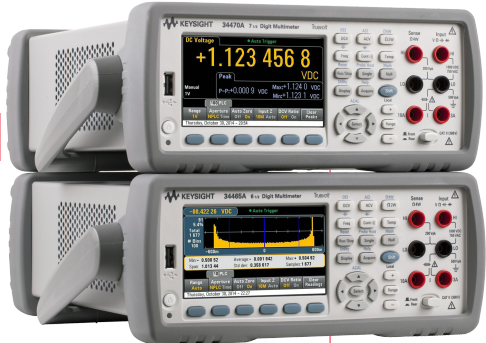
\includegraphics[width=0.3\textwidth]{Chap06/Figures/DMM_34460A.PNG}}
	\caption{ keysight N6705 Power Supply and DMM 34460A }
	\label{fig:keysight_n6705_DMM_34460A}
\end{figure}

\begin{figure}[h]
	\centering
	\subfigure[16CH Battery Cell Simulator 87001]{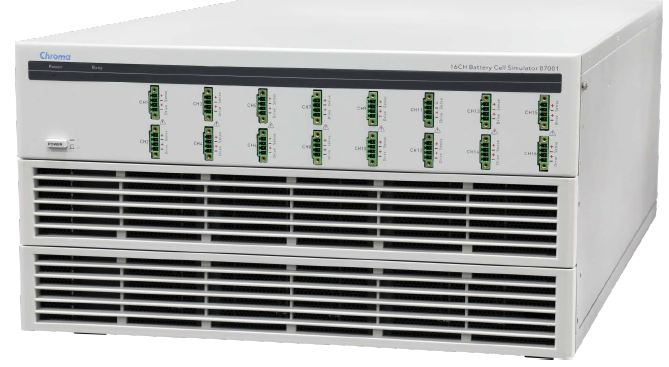
\includegraphics[width=0.3\textwidth]{Chap06/Figures/Chroma.PNG}}
    \qquad
	\subfigure[Chroma Output Wiring to the BMS]{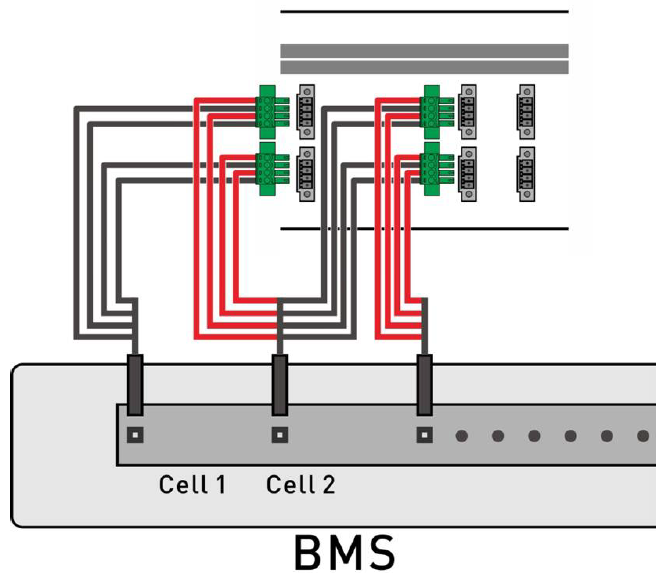
\includegraphics[width=0.3\textwidth]{Chap06/Figures/Chroma_Output_wiring.PNG}}
	\caption{16CH Battery Cell Simulator 87001}
	\label{fig:Chroma}
\end{figure}

